\message{ !name(thesis.tex)}\documentclass[11pt,Chicago]{uuthesis}

% SETUP
\usepackage{amssymb}
\usepackage{graphicx}
%\DeclareGraphicsExtensions{.jpg,.png}
\usepackage{amsmath}
\usepackage[utf8]{inputenc}
\usepackage{listings}
\usepackage{hyperref}
\hypersetup{
    colorlinks,
    citecolor=black,
    filecolor=black,
    linkcolor=black,
    urlcolor=black
}
\fourlevels
\setcounter{tocdepth}{4}
\addtocontents{toc}{\protect\sloppy}

% INFO
\title{Modeling Concurrency:\protect\\Extending SMACK to Support Pthreads}
%Supporting pthreads in SMACK verifier
%Pthreads extension for SMACK verifier
\author{Montgomery Carter}
\supervisor{Zvonimir Rakamarić}
\submitdate{May 2015}
\copyrightyear{2015}
\thesistype{thesis}

% DOCUMENT
\begin{document}

\message{ !name(thesis_background.tex) !offset(-35) }
\chapter{Background}
Developing a full featured software verification tool from end-to-end can be a daunting task.  Bounded model checking requires several steps.  First, the input source code must be parsed or compiled.  The resulting abstract syntax tree (AST) must then be semantically interpreted, and a model built of underlying program semantics.  Finally, the modeled program must be represented as an SMT query and passed through an SMT solver.  This imposes a large barrier to entry for prototyping a new model checking algorithm, or building a verification tool for a new source language using existing algorithms.

The Boogie intermediate verification language (IVL) was designed to alleviate the complexity of modeling new source languages and implementing new model checking algorithms.  Boogie IVL separates the task of modeling input program semantics from the task of bounding and checking modeled programs.  This allows model checking tools to take Boogie IVL files as input, rather than the input source language.  Similarly, front-end tools can translate to Boogie IVL rather than being directly integrated with the model checker.  By providing a clear, distinct interface between the two tasks, Boogie IVL [allow for modular tool components rather than end-to-end verification tools].

Due to its goal of creating an abstraction between program modeling and model checking, Boogie IVL has been designed to be a very low-level modeling language.  It contains support for little more than a typing system, basic arithmetic and boolean expressions \& statements, control flow \& procedure calls, and verification condition specification~\cite{boogie}.  Any more complicated semantics of the source language must be modeled using the basic set of primitives available in Boogie IVL.

Though the low-level nature of Boogie IVL provides the flexibility to support a large variety of models of computation and source languages, it requires that models be created to define the semantics of operations available within the source language and computational model environments.  As an example, there is no concept of a heap within Boogie.  Because of this, a memory model must be developed that accurately models the behavior of the heap.  A rudimentary model of memory could use a simple, large array of integers to represent the heap, where each element represents a word of memory, and C pointers are simply indices into this array.

There are several back-end model checking tools that support 

SMACK itself is essentially a compiler that takes C/C++ programs and translates them into BoogiePL (or simply Boogie), an intermediate verification language (IVL)~\cite{smack}.  This converted Boogie code is then consumed by a static analysis tool that evaluates verification conditions present in the original source code.

The SMACK toolchain is depicted in Figure~\ref{fig:SMACKToolchain}.  SMACK as a whole is a front-end for a program verification toolchain that features the Corral program verifier as its core back-end.  Input C/C++ programs are given to Clang to compile and link, resulting in an LLVM bytecode output.  This is then passed to the SMACK executable, which translates the LLVM bytecode into a Boogie program that models the behavior of the input C/C++ program.  The resulting Boogie program is then passed to Corral.  Corral converts the Boogie program into an SMT query, which is given to the Z3 SMT solver for evaluation.

\begin{figure}[h]
  \caption{SMACK Toolchain}
  \label{fig:SMACKToolchain}
  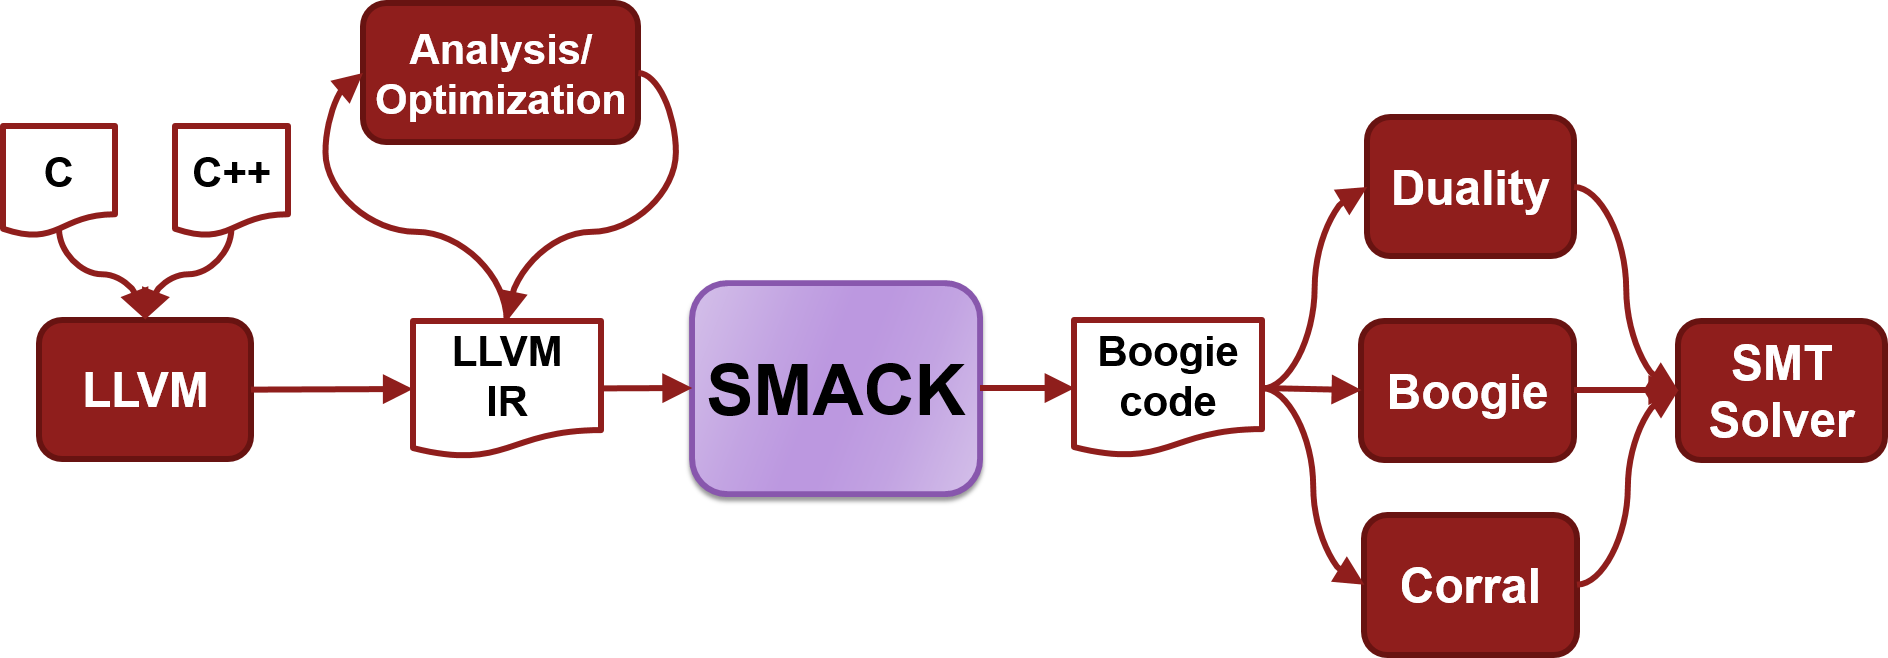
\includegraphics[width=1\textwidth]{SmackToolchain.png}
\end{figure}

[Does this belong somewhere else?] It should be noted that there exists a back-end verifier from Microsoft Research named Boogie.  The Boogie program verifier provides similar functionality to the Corral program verifier.  Hereafter, ``Boogie'' will refer to BoogiePL unless otherwise specified.

The Corral program verifier provides an extension to the Boogie language that includes a very basic set of primitives for handling concurrency.  This extension includes the following calls:
\begin{itemize}
\item \lstinline|async call| \emph{func}\lstinline|(|\emph{...}\lstinline|)| - Asynchronously calls \emph{func} with the parameter list \emph{'...'}
\item \lstinline|corral_atomic_begin()| - Begins an atomic block
\item \lstinline|corral_atomic_end()| - Ends an atomic block
\item \lstinline|corral_getThreadID()| - Returns the ID of the calling thread.
\item \lstinline|corral_getChildThreadID()| - Returns the ID of the thread most recently spawned in the calling procedure.
\end{itemize}
The Pthreads API is much more complex than these concurrency primitives recognized by Corral.  As a result, to provide support for the more complex Pthreads API within SMACK, it is necessary to model the behavior of the Pthreads API using the primitives provided by Corral.

There are several projects, including Inspect and CIVL, that provide support for Pthreads~\cite{civl}\cite{inspect}.  I will be referring to their implementations, as well as using their benchmarks and regression tests to assess the accuracy of the new implementation within SMACK.
%%% Local Variables: 
%%% mode: LaTeX
%%% TeX-master: "thesis"
%%% End: 

\message{ !name(thesis.tex) !offset(-15) }

\end{document}

%%% Local Variables:
%%% TeX-master: "thesis"
%%% End: